\documentclass[sigconf,anonymous,review]{acmart}
\setcopyright{none}
\settopmatter{printacmref=false}
\renewcommand\footnotetextcopyrightpermission[1]{}
\acmConference[AI-Driven Markets '26]{AI-Driven Market Microstructure in Centralized and Decentralized Finance}{November 2026}{Milan, Italy}
\acmYear{2026}
\title{Risk and Turnover Preferences in Learned Portfolio Rebalancing}
\author{Anonymous Author(s)}
\newcommand{\E}{\mathbb{E}}
\newcommand{\Var}{\operatorname{Var}}
\newcommand{\Cov}{\operatorname{Cov}}
\newcommand{\eq}{\mathrm{eq}}
\newtheorem{proposition}{Proposition}
\newtheorem{theorem}{Theorem}
\begin{document}
\begin{abstract}
Risk and turnover penalties jointly determine the trades selected by a portfolio reward. Replacing variance with a second moment changes this trade-off, even when the risk coefficient is subsequently calibrated. For a constrained one-period allocator, we derive the additional turnover penalty introduced by risk-only calibration and show that jointly scaling risk and cost coefficients preserves the mean--variance optimum. The result follows the standard mean auxiliary and is verified against an adapted MVPI solver. A walk-forward study of ten US industry portfolios over 1990--2025 compares induced allocations on common pre-trade states and realised returns on separate strategy paths. Joint calibration recovers the fitted policy across 17 settings; scalar and risk-only adjustments retain discrepancies. Realised performance differences are inconclusive, and finite-budget policy optimisation introduces a larger error than the primary reward-design gap. The study provides an interpretable test of risk--cost preferences in trading models, with monthly proportional costs rather than an order-book or market-impact model.
\end{abstract}
\ccsdesc[500]{Computing methodologies~Reinforcement learning}
\ccsdesc[300]{Applied computing~Economics}
\keywords{portfolio allocation, reward alignment, mean--variance, reinforcement learning, transaction costs}
\maketitle

\section{Introduction}
A trading reward balances the incentive to take risk against the incentive to trade. These incentives are often assigned separate coefficients, yet changing one part of the reward can alter the effective meaning of the other. In particular, replacing a variance penalty with a squared-return penalty and then recalibrating risk need not preserve the intended turnover preference.

This paper studies that interaction in constrained portfolio rebalancing. On each estimated market state, the intended reference is mean return minus covariance risk and proportional turnover cost. We compare it with second-moment rewards, scalar calibrations and a log-minus-variance preference adapted from Jiang et al.\ \cite{jiang2025}. All local comparisons face the same pre-trade portfolio.

An auxiliary-variable identity makes the distortion explicit. Risk-only calibration adds a turnover term whose magnitude depends on the target expected return. Joint risk--cost calibration removes it and agrees with an adapted MVPI method\ \cite{zhang2021}. Historical data then show how this exact fitted relation differs from realised investment performance.

The setting addresses the robustness and interpretation of AI trading objectives. It uses monthly industry portfolios and a first-order proportional cost approximation. It therefore identifies a reward-level source of preference drift before adding execution dynamics; it does not estimate market impact, liquidity provision or order-book behaviour.

\section{Portfolio objectives and validation}
Direct utility optimisation is established in financial learning. Simon et al.\ \cite{simon2026}, Section 4.1, Eq.\ (17), use centred mean--variance preferences, with turnover costs in Section 3.6. Their deep portfolio policy and US stock-characteristic data differ from the common industry-portfolio environment used here. Cong et al.\ \cite{cong2026}, Eqs.\ (19)--(20), optimise trajectory objectives through pathwise gradients. These approaches show that objective-aware learning is feasible.

Other rewards encode different preferences. Jiang et al.\ \cite{jiang2025}, Eq.\ (8), use net log return minus a variance penalty; Eq.\ (19) adds trading restrictions. We adapt that preference using monthly returns, hard simplex constraints and a first-order turnover charge. The comparison changes the reward while holding the estimated state fixed; it does not reproduce their CNN/WaveNet DPG system. Their earlier TD3 study\ \cite{jiang2024}, Eq.\ (4), combines portfolio value, variance and trading costs, motivating explicit treatment of all three terms.

The calibration below follows the mean auxiliary in MVPI\ \cite{zhang2021}. Known-policy validation also has precedents: Chaouki et al.\ \cite{chaouki2020}, Section 3, compare learned and analytical controls, while Gollart and Okhrin\ \cite{gollart2025}, Section 4.2.1 and Table 1, align terminal utility with a DDPG problem. Our contribution is a reproducible test of risk--cost preference drift and a comparison of its magnitude with optimisation error and historical uncertainty.

\section{Constrained alignment with turnover costs}
Let $m$ and $\Sigma\succ0$ be estimated excess-return moments available before trading, $M=\Sigma+mm^\top$, and $\nu=m^\top M^{-1}m$. The feasible set $C$ is the simplex, $p$ is the pre-trade allocation, and $c(u)=\|u-p\|_1$. For risk aversion $\varphi>0$ and cost coefficient $\lambda\ge0$, define
\begin{equation}\label{eq:target}
 F(u)=m^\top u-\varphi u^\top\Sigma u-\lambda c(u),\quad u\in C.
\end{equation}
Its unique optimum $u^*$ is a \emph{fitted reference}, not the unknown true market optimum. The reference specifies a one-period decision under estimated moments.

\begin{proposition}\label{prop:joint}
Let $y^*=m^\top u^*$ and $A=1+2\varphi y^*>0$. The second-moment reward objective
\begin{equation}
 Q(u)=m^\top u-\frac{\varphi}{A}u^\top M u-\frac{\lambda}{A}c(u)
\end{equation}
has the same unique maximiser as $F$.
\end{proposition}
\begin{proof}
For all feasible $u$,
\begin{equation}\label{eq:identity}
 AQ(u)=F(u)-\varphi(m^\top u-y^*)^2+\varphi(y^*)^2.
\end{equation}
At $u^*$ the square vanishes and $F$ is maximal. Since $A>0$, the assertion follows.
\end{proof}
The argument applies to any feasible set with a global maximiser. Convexity and positive definite covariance ensure uniqueness here. The identity follows the mean auxiliary used in MVPI\ \cite{zhang2021}.

If only the risk coefficient is divided by $A$, while the cost coefficient stays $\lambda$, the right-hand side of Eq.\ \eqref{eq:identity} gains the extra term
\begin{equation}\label{eq:costdistortion}
 -2\varphi y^*\lambda c(u).
\end{equation}
When $y^*>0$, this increases the effective cost preference. It need not imply monotone realised turnover on the strategy's evolving path. The unconstrained formula $\varphi(1-\nu)$ likewise need not calibrate a constrained optimum.

Joint calibration uses $u^*$ and therefore serves as a certificate of alignment with a known reference. As a constructive prior-art comparator, we also alternate maximising
\begin{equation}
 (1+2\varphi y)m^\top u-\varphi u^\top Mu-\lambda c(u)
\end{equation}
and setting $y=m^\top u$. This is an adaptation of the MVPI mean auxiliary to the constrained one-period problem. Including the term $-\varphi y^2$ gives a jointly strictly concave objective, since its quadratic block has Schur complement $\Sigma\succ0$. Exact block updates converge to the same target. This provides a constructive comparator with the same optimum.

\section{Historical study}
\subsection{Data and protocol}
We use Kenneth French's ten value-weighted US industry portfolio monthly total returns and the Fama--French risk-free series\ \cite{french}. The archived downloads have a recorded SHA-256 manifest. Estimation data start January 1970; evaluation covers January 1990--December 2025 (432 months). This is a retrospective study on the August 2026 revised vintage, not a point-in-time constituent dataset. Industry portfolios are research portfolios, not directly tradeable funds; their internal reconstruction costs are not included. The provider's CRSP processing and risk-free source changes also form part of this data vintage.

For month $t$, use only the previous 120 months of excess returns to estimate $m$ and the unbiased covariance, shrunk 10\% toward its diagonal. All strategies are long-only and fully invested. The primary settings are $\varphi=5$ and $\lambda=0.001$ (10 basis points per unit of L1 turnover). Pre-trade weights drift with realised gross asset returns. Net portfolio return uses the explicit first-order convention $u_t^\top R_t-\lambda\|u_t-p_t\|_1$, not a market-impact model or exact intramonth execution equation. The experimental protocol fixed these choices before strategy outcomes were inspected.

\subsection{Comparators and measurements}
We solve the covariance-MV target, raw second moment ($\kappa=\varphi$), unconstrained scalar calibration ($\kappa=\varphi(1-\nu)$), reference-based risk-only calibration, joint calibration, and MVPI adaptation. Equal weight and minimum variance provide conventional portfolio controls. Log utility and log-minus-variance adapt the reward preference in Jiang et al.\ \cite{jiang2025}; every method uses the same monthly data and feasible set. The comparison tests induced preferences under common estimates, not which published learning architecture is best.

For alignment, all methods face the target strategy's \emph{same pre-trade state}. We report Euclidean allocation distance and fitted regret $F(u^*)-F(u)$. Each strategy also follows its own pre-trade states for realised performance. This avoids conflating state divergence with the local reward comparison. Quadratic solutions have independent linear-programme first-order certificates; the largest saved common-state certificate is $4.27\times10^{-9}$ in objective units. The observed agreement of calibrated policies is considerably tighter than the acceptance tolerance.

Realised metrics are monthly excess-return MV, annualised excess Sharpe, return, volatility, turnover and drawdown. Uncertainty for paired MV differences uses 1,000 circular moving-block bootstrap resamples, blocks of 12 months, seed 8128. These intervals describe the observed strategy-return sequences, not full estimator-refitting or model-selection uncertainty. Robustness spans 17 prespecified combinations: $\varphi\in\{2,5,10\}$ and cost $\{0,10,25\}$ bp at the primary estimator, plus windows $\{60,120,240\}$ and covariance shrinkage $\{0,0.1,0.5\}$ at the primary preferences. The overlapping primary case is counted once.

\begin{table*}[t]
\centering
\caption{Primary historical comparison, 1990--2025. Distance and fitted regret use common states; realised metrics use each strategy's own path. Gap and MV score are monthly basis-point units. Calibration improves model alignment; the table does not establish superior investment performance.}
\label{tab:historical}
\begin{tabular}{lrrrr}\toprule
Method & Mean allocation distance & Fitted MV gap (bp) & Excess Sharpe & Realised MV (bp)\\\midrule
Target & 0.00000 & 0.0000 & 0.570 & -8.497 \\
Raw second moment & 0.00843 & 0.0148 & 0.573 & -7.182 \\
Unconstrained scalar & 0.00540 & 0.0043 & 0.568 & -8.882 \\
Risk-only calibration & 0.00510 & 0.0033 & 0.571 & -8.365 \\
Joint calibration & 0.00000 & 0.0000 & 0.570 & -8.497 \\
MVPI adaptation & 0.00000 & 0.0000 & 0.570 & -8.497 \\
Log minus variance & 0.01286 & 0.0287 & 0.572 & -7.123 \\
Log utility & 0.54848 & 39.7855 & 0.344 & -133.295 \\
Equal weight & 0.43495 & 46.2626 & 0.622 & -11.893 \\
Minimum variance & 0.23843 & 9.0252 & 0.645 & 5.274 \\
\bottomrule\end{tabular}

\end{table*}

\subsection{Results}
Table~\ref{tab:historical} shows that raw second-moment optimisation has mean allocation distance 0.00843. Unconstrained scalar calibration reduces this to 0.00540; reference-based risk-only calibration retains 0.00510. Joint calibration and MVPI agree with the fitted reference to numerical precision. The adapted log-minus-variance objective has distance 0.01286; log utility alone is much farther away. The differences measure departure from the specified MV preference; log utility represents a different investment objective.

Across all 17 settings, the largest mean joint-calibration distance is $1.54\times10^{-7}$; raw mean distances range from 0.00157 to 0.03682. Thus constraints and trading costs do not break the joint identity, while unconstrained scalar calibration is not a universal repair. Figure~\ref{fig:historical} relates alignment to historical outcomes, and Figure~\ref{fig:robust} gives robustness and uncertainty.

Joint calibration has realised monthly MV lower than raw by 1.315 bp, with 95\% interval $[-3.318,0.343]$ bp. Against scalar calibration the difference is 0.385 bp. Its interval is $[-0.570,1.351]$ bp. Against risk-only calibration the difference is $-0.131$ bp, with interval $[-0.889,0.634]$ bp. All include zero. Minimum variance has both a better realised MV score and higher Sharpe than the fitted target in the primary sample. This illustrates estimation risk: precise implementation of estimated preferences cannot guarantee the best realised allocation. Equal weight has higher Sharpe than the target but lower realised MV, so Sharpe ranking alone does not answer even the ex-post MV comparison.

\begin{figure*}[p]
\centering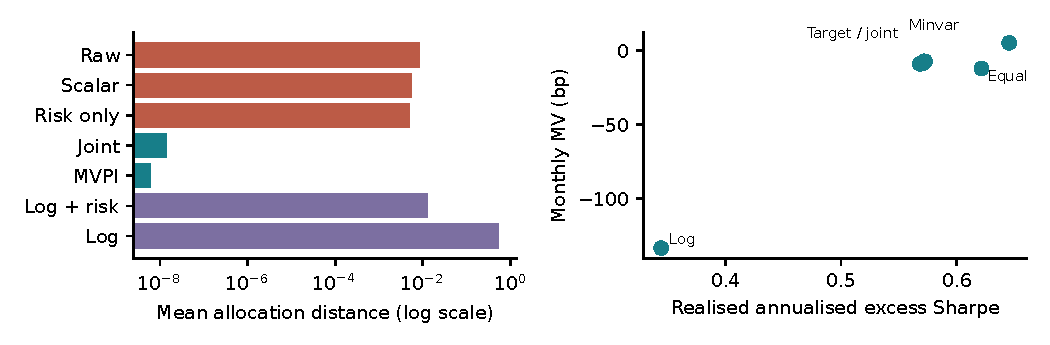
\includegraphics[width=.94\textwidth]{figures/historical.pdf}
\caption{Left: mean common-state allocation distance; the logarithmic axis exposes numerical agreement for joint calibration and MVPI. Right: realised Sharpe and monthly MV need not rank policies alike. Equal weight has higher Sharpe but lower MV than the fitted target.}
\Description{Allocation distances on the left and realised Sharpe versus mean-variance on the right.}
\label{fig:historical}
\end{figure*}
\begin{figure*}[p]
\centering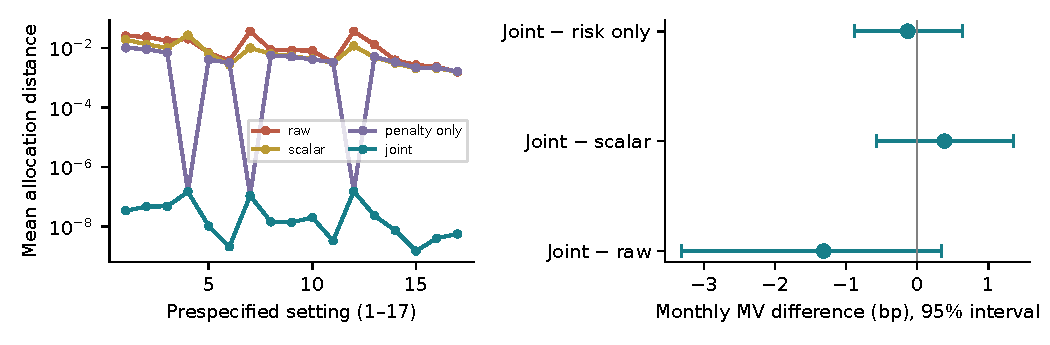
\includegraphics[width=.94\textwidth]{figures/robustness.pdf}
\caption{Left: alignment across the 17 prespecified settings, ordered by window, risk penalty, cost and shrinkage. Right: paired 12-month-block bootstrap intervals all include zero. Exact fitted alignment does not imply a statistically clear realised MV advantage.}
\Description{Seventeen-setting allocation-distance curves and three paired confidence intervals crossing zero.}
\label{fig:robust}
\end{figure*}

\subsection{Separating optimisation from reward design}
A finite-budget experiment assigns independent softmax policy logits to each of the 432 historical common states. Adam uses learning rate 0.05, initial logits $N(0,0.1^2)$, five matched seeds and 50, 250, 1,000 and 5,000 gradient steps. Each objective uses only its state's lagged estimates. Independent logits isolate optimisation error on each fitted state. They do not test generalisation across states, as a predictive neural policy would.

Let $u_r$ maximise the specified reward and $\widehat u_r$ be the finite-budget allocation. We report the nonnegative own-reward optimisation gap separately from
\begin{align}
 F(u^*)-F(\widehat u_r)
 &= [F(u^*)-F(u_r)]\nonumber\\
 &\quad+[F(u_r)-F(\widehat u_r)].
\end{align}
The second bracket is a \emph{signed} target-value difference; it is not the own-reward optimisation gap. At 5,000 steps, mean own-reward optimisation gaps remain approximately $4\times10^{-6}$, exceeding the exact raw design gap of $1.48\times10^{-6}$. Thus finite-budget error can dominate the reward discrepancy. Figure~\ref{fig:learning} shows why these must be kept separate: improving the raw-reward optimiser does not remove its exact design gap. The target and joint reward have the same limiting optimum but can exhibit different finite-budget trajectories because their objective geometries differ.

\begin{figure*}[p]
\centering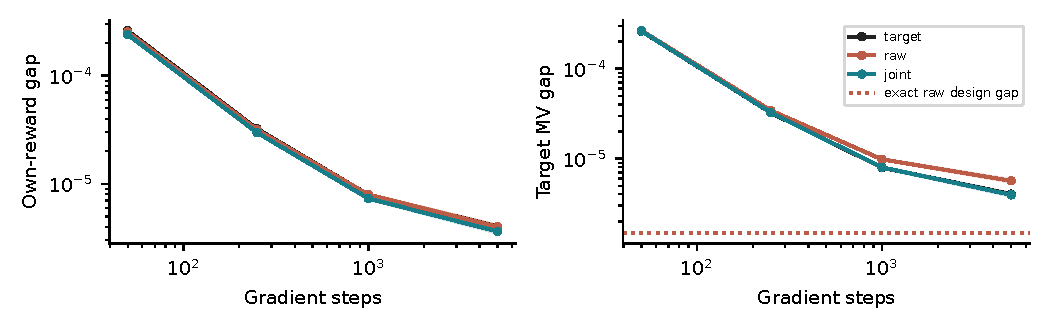
\includegraphics[width=.94\textwidth]{figures/learning.pdf}
\caption{Finite-budget softmax optimisation on historical fitted states. Lines are five-seed means, shading the seed range. Left uses each method's own reward; right uses the common MV target. The dotted line is the exact raw reward-design gap. This diagnostic measures optimisation accuracy, not generalisation.}
\Description{Own-reward and target gaps decline with gradient steps; the raw target gap remains above its design floor.}
\label{fig:learning}
\end{figure*}

\section{Reconstructing the historical experiment}
\subsection{Information available at a decision}
Write $R_t\in\mathbb R^{10}$ for the vector of monthly total returns and $r_{f,t}$ for the risk-free return. For a window of length $L$, the information used at month $t$ is $\{R_s,r_{f,s}:t-L\le s<t\}$. In particular, neither $R_t$ nor a full-sample covariance enters the allocation. Let $X_s=R_s-r_{f,s}\mathbf1$. The sample mean and covariance are
\begin{align}
 m_t&=L^{-1}\sum_{s=t-L}^{t-1}X_s,\\
 S_t&=(L-1)^{-1}\sum_{s=t-L}^{t-1}(X_s-m_t)(X_s-m_t)^\top.
\end{align}
The implemented covariance is $\Sigma_t=(1-h)S_t+h\operatorname{diag}(S_t)$, with $L=120$ and $h=0.1$ in the primary experiment. The mean is not shrunk. Thus every reward sees identical estimates; differences are not attributable to different forecasting models. Positive definiteness is checked before optimisation. Historical dependence can be present in the observed returns without changing the algebra on a fixed estimated state. It does change how much confidence one should place in that estimated state as a forecast.

The raw files contain percent returns, which are divided by 100 before any objective is evaluated. Monthly records are aligned by date; missing-value sentinels, duplicate dates and missing joined observations are rejected. Estimation data begin in 1970 to support the longest 240-month window at the first 1990 decision. Observations after December 2025 are excluded even though the retrieved files extend further. The saved date range therefore fixes the comparison independently of the most recent available month.

\subsection{Two uses of the same historical month}
The alignment calculation and the investment calculation answer different questions. For alignment, all rewards receive the reference strategy's pre-trade portfolio $p_t^*$. Define $u_t^*$ as the fitted target allocation and $u_t^r$ as the allocation induced by reward $r$ on that common state. We record
\begin{equation}
 d_t^r=\|u_t^r-u_t^*\|_2,\qquad
 g_t^r=F_t(u_t^*)-F_t(u_t^r).
\end{equation}
The first measures the change in portfolio weights, while the second measures the economic cost under the stated fitted preference. A small objective gap can accompany a visible weight difference when the objective is locally flat. Neither quantity uses the month's subsequent realised return.

For investment performance, each method instead carries its own pre-trade portfolio $p_t^r$. It solves its reward again on that state, giving $\bar u_t^r$. The recorded turnover and net return are
\begin{equation}
 T_t^r=\|\bar u_t^r-p_t^r\|_1,\qquad
 r_t^r=(\bar u_t^r)^\top R_t-\lambda T_t^r.
\end{equation}
All methods start from equal weights. Before the next decision, holdings drift according to
\begin{equation}
 p_{t+1,i}^r=
 \frac{\bar u_{t,i}^r(1+R_{t,i})}{1+(\bar u_t^r)^\top R_t}.
\end{equation}
This uses gross asset returns to update relative holdings and subtracts costs separately in the first-order portfolio-return approximation. Charging exact self-financing costs would require a different wealth-accounting model. Using each method's own holdings in the alignment calculation would mix reward disagreement with the consequences of earlier decisions; the common-state record avoids that confounding.

\subsection{What the published baselines represent}
The MVPI comparator implements the mean auxiliary of Zhang et al.\ \cite{zhang2021} in the constrained one-period setting. Starting from $y=0$, it alternates a portfolio maximisation with the update $y\leftarrow m^\top u$. The portfolio step retains the original turnover coefficient. The procedure stops when the change in $y$ is below $10^{-10}$, with a maximum of 200 iterations. It computes the reference without first inserting the reference allocation into the reward. Joint calibration, by contrast, uses the already computed reference mean to demonstrate exact alignment. Their numerical agreement is a consistency check between two constructions, not an advantage over MVPI.

The Jiang et al.\ \cite{jiang2025} adaptation maximises
\begin{equation}
 \frac1L\sum_{s=t-L}^{t-1}\log(1+u^\top R_s)
 -\varphi u^\top\Sigma_tu-\lambda\|u-p_t\|_1.
\end{equation}
Setting its variance coefficient to zero gives the log-utility comparator. Logarithmic utility uses total returns, while the fitted MV objective uses excess returns. Both formulations receive the same historical window and feasible set. This is a deliberate comparison of preferences: logarithmic utility is not an algebraic approximation to the specified MV target. Hard simplex constraints and the linear turnover charge replace the source paper's soft restrictions and log cost factor. Its published returns are not pooled with ours, and its predictive architecture is not evaluated.

Equal weight supplies a fixed-allocation control. The minimum-variance control removes the expected-return term from the fitted target while retaining the risk scaling and turnover charge. It therefore tests whether using the estimated mean helps realised performance under this protocol. Its strong primary outcome is evidence that estimation quality matters even when reward alignment is exact.

\subsection{Numerical and statistical resolution}
Quadratic objectives are solved with auxiliary variables $z_i\ge |u_i-p_i|$ and simplex constraints. The implemented minimisation is scaled for numerical conditioning, but certificates are computed in the original objective units. Given a feasible iterate $x$ in the extended polytope $\mathcal P$, a separate linear programme gives the certificate
\begin{equation}
 C(x)=\max_{v\in\mathcal P}\nabla f(x)^\top(x-v),
\end{equation}
where $f$ is the convex negative reward. Convexity implies $f(x)-\min f\le C(x)$. This checks accuracy independently of the quadratic optimiser's success flag. Poorly certified iterates are retried at different scales and rejected if the certificate remains above $2\times10^{-7}$. The log comparators use a separate concave optimisation problem; the quadratic certificate is not claimed for them.

Realised monthly MV is the sample mean of net excess returns minus $\varphi$ times their sample variance. Excess Sharpe annualises the monthly mean-to-standard-deviation ratio by $\sqrt{12}$. These are evaluated on each strategy's complete own-state return path. For paired MV uncertainty, the same circular 12-month blocks are sampled for both strategies, with 1,000 repetitions and seed 8128. Shared blocks retain contemporaneous dependence between strategies and some serial dependence within each path. The intervals condition on the fitted strategies' realised paths: they do not repeat estimation, select hyperparameters or quantify every source of model uncertainty.

\section{Interpreting calibration across settings}
\subsection{Which comparison can establish improvement?}
A calibration rule is evaluated against a stated financial preference. In this study, improvement in alignment means a smaller $d_t^r$ or $g_t^r$ on the same estimated state. It does not mean that the calibrated strategy earns a higher return in the next month. The realised ranking can reverse because the target's estimated mean and covariance are imperfect forecasts. This distinction is especially relevant when the target itself uses a noisy expected-return estimate and a competing policy happens to reduce exposure to that estimate.

The primary distances put the scale of the comparison in context. Raw second moments give mean Euclidean distance 0.00843; unconstrained scalar calibration reduces it to 0.00540; reference-based risk-only calibration gives 0.00510. Joint calibration and the MVPI adaptation agree with the target to numerical precision. The log-minus-variance adaptation has distance 0.01286. These are distances between ten-dimensional weight vectors, not percentages of portfolio wealth lost. Fitted regret supplies the corresponding objective scale: the raw reward gap is only 0.0148 monthly basis points. A statistically visible allocation difference can therefore be economically small under the fitted preference.

The historical MV score answers a different question. Joint calibration is 1.315 monthly basis points below raw in the primary sample, while its interval spans both signs. That result does not support a claim that the calibrated policy is a superior investment strategy. Nor does it disprove the calibration identity: subsequent realised returns are absent from that identity. Minimum variance's better realised MV and Sharpe suggest that a strong practical implementation would need to address estimation quality alongside reward design.

\subsection{What the robustness grid tests}
The first block crosses three risk coefficients, $\varphi\in\{2,5,10\}$, with three turnover charges, $\lambda\in\{0,0.001,0.0025\}$, at the primary estimation window and shrinkage. The second crosses $L\in\{60,120,240\}$ with $h\in\{0,0.1,0.5\}$ at the primary risk and cost coefficients. Their shared primary setting is counted once, giving 17 distinct specifications. This is a union of two grids rather than the full cross-product of every choice. It probes economically relevant perturbations without pretending to span all market models.

The maximum setting-mean distance for joint calibration is $1.54\times10^{-7}$, compared with raw mean distances ranging from approximately 0.00157 to 0.03682. This supports the identity across the evaluated covariance estimates, constraints and cost levels. It does not supply 17 independent statistical replications: all settings reuse the same asset universe and overlapping return observations. The robustness runs compare the target, raw, scalar, risk-only, joint, equal-weight and minimum-variance policies. The MVPI and logarithmic comparators are evaluated in the primary study, rather than silently treated as rerun throughout this grid.

At zero transaction cost the risk-only and joint reward definitions coincide. With positive cost, the difference depends on the target expected return through $A=1+2\varphi y^*$. Constraints can make distinct objectives select the same boundary allocation, so exact agreement at an individual state need not establish equivalence of the rewards at all states. Conversely, a small discrepancy at the primary setting cannot be assumed to remain small when risk, cost or estimation changes.

\subsection{Optimisation effort and reward fidelity}
The finite-budget comparison assigns independent logits to each historical state. Softmax enforces strictly positive weights at finite logits, so exact boundary allocations can be approached without being attained. This helps explain why a high-accuracy constrained solver and a finite-budget softmax optimiser need not have equal residual errors even on the same objective. All three trained objectives use identical initialisation distributions, seeds and step budgets; the diagnostic compares numerical effort under that common parameterisation.

The own-reward gap measures whether the optimiser solved the reward it was given. The signed transfer term in the target decomposition instead measures how the approximate policy changes the target value relative to the exact reward optimum. It can have either sign. Adding own-reward suboptimality directly to target-unit design regret would mix different objective scales and would not reproduce the total target gap. At 5,000 steps, mean own-reward gaps remain around $4\times10^{-6}$, larger than the exact raw design gap of $1.48\times10^{-6}$. Improving the optimiser can therefore be the larger immediate numerical intervention, while calibration addresses the distinct discrepancy that persists at exact optimisation.

\section{Risk and trading-cost coefficients as joint preferences}
\subsection{A local interpretation of a second-moment reward}
Consider the reward $Q(u)=m^\top u-\kappa u^\top Mu-\eta c(u)$, with a positive quadratic coefficient $\kappa$ and raw cost coefficient $\eta$. At an optimum $\hat u$, choose a turnover subgradient $s\in\partial c(\hat u)$. Its reward gradient, including that subgradient, can be written
\begin{equation}
 (1-2\kappa m^\top\hat u)m-2\kappa\Sigma\hat u-\eta s.
\end{equation}
If $b=1-2\kappa m^\top\hat u>0$, division by $b$ identifies sufficient effective MV coefficients
\begin{equation}
 \varphi_{\mathrm{eff}}=\kappa/b,\qquad
 \lambda_{\mathrm{eff}}=\eta/b.
\end{equation}
The normal cone of the feasible set is unchanged by positive scaling, so the constrained first-order optimality condition is also the condition for these effective preferences. Concavity makes that condition sufficient. The interpretation requires $b>0$; it is not extended to a nonpositive denominator. Active constraints can also make several coefficient pairs select the same portfolio, so the inverse interpretation need not be unique.

This calculation explains why tuning a second-moment coefficient changes more than the apparent risk aversion. The effective turnover coefficient is rescaled through the selected expected return. Holding the raw cost number fixed while changing $\kappa$ does not generally hold the economic trading preference fixed. A comparison that labels every reward with the same nominal transaction-cost parameter can therefore still compare different induced trading preferences.

\subsection{The meaning of turnover in this experiment}
For fully invested long-only weights, the L1 distance counts both purchases and sales. A transfer of weight $\delta$ from one industry to another contributes $2\delta$ to $\|u-p\|_1$. Accordingly, the primary coefficient is explicitly 10 basis points per unit of L1 turnover; it should not be read as 10 basis points per one-way transfer. Keeping this convention fixed across methods is necessary for a fair comparison.

The reference-based risk-only reward adds the term $-2\varphi y^*\lambda c(u)$ after conversion into target units. When $y^*>0$, this favours staying closer to the pre-trade portfolio relative to the correctly rescaled objective. That is a statement about the reward on a fixed state. It is not a theorem that realised turnover is always lower over an entire historical path: different earlier positions alter future trade requirements, and constraints can change which assets are held. The experiment therefore measures turnover on each method's own path while auditing preference distortion on a shared state.

The model treats industry returns as unaffected by the strategy's allocations. It contains neither a limit-order book nor endogenous price impact, fill probabilities or a choice of execution time. The proportional charge is useful for isolating a reward-design mechanism, but it does not identify a capacity limit or an optimal execution schedule. An execution study would need to specify those additional states and decisions before deciding which financial objective the reward should preserve.

\subsection{A reusable check for trading-model comparisons}
A practical comparison begins by writing every reward in the same return and turnover units. Next, it fixes the information set and feasible trades at a common state. Solving the stated target and each proposed reward then reveals whether changes in risk and cost coefficients alter the intended trade-off. The certificate and target-regret records distinguish an economic difference from solver noise. Only after that comparison should realised paths be used to discuss return, drawdown or turnover.

This procedure is particularly helpful when a reward is modified by normalisation, rescaling or an auxiliary variable. Multiplying the entire objective by a positive constant preserves its optimum. Scaling only one term generally does not. The joint identity provides an exact instance of this principle for the present covariance-MV problem. Applying it to state-dependent execution costs, inventory constraints or endogenous impact would require a new derivation; the monthly evidence here supplies a controlled example of what should be checked.

\section{Realised rebalancing and chronological outcomes}
The aggregate alignment measures do not describe the size of the trades made along each strategy's own path. Table~\ref{tab:trades} reports average monthly L1 turnover together with annualised arithmetic net return and maximum drawdown. Turnover is expressed as a percentage of portfolio weight, not as the fraction of one-way purchases. The return annualisation multiplies the monthly arithmetic mean by twelve; it is not a compound annual growth rate.
\begin{table}[ht]
\centering\small
\caption{Own-path trading and return summaries, 1990--2025. Turnover is mean monthly L1 turnover (\%); return is annualised arithmetic net return (\%); drawdown is the largest wealth decline (\%).}
\label{tab:trades}
\begin{tabular}{lrrr}\toprule
Method & Turnover & Return & Drawdown\\\midrule
Target / joint & 2.29 & 10.07 & -41.89 \\
Raw & 2.04 & 10.01 & -41.02 \\
Scalar & 2.15 & 10.07 & -42.75 \\
Risk only & 2.11 & 10.08 & -42.44 \\
Equal weight & 2.54 & 11.64 & -48.09 \\
Minimum variance & 0.86 & 10.32 & -35.42 \\
Log + variance & 2.18 & 9.99 & -40.72 \\
\bottomrule\end{tabular}
\end{table}
A smaller fitted reward gap does not order these path statistics. The target and joint rewards implement the same fitted preference, but comparisons with raw or scalar rewards also reflect different holdings carried from previous months. The first-order cost convention charges the same coefficient to all realised paths, including the path generated by a reward whose \emph{effective} cost preference differs. This keeps realised accounting distinct from the incentive encoded in the reward.

Table~\ref{tab:periods} breaks the existing paths into three chronological intervals. No strategy is restarted at a boundary, and the estimation window continues to roll through prior observations. The rows describe sample variation within the same experiment; they are not independent training and test replications. The paired primary uncertainty calculation uses the full period, so no separate significance claim is attached to these shorter summaries.
\begin{table}[ht]
\centering\small
\caption{Chronological own-path outcomes. MV is monthly basis points; Sharpe uses monthly net excess returns and $\sqrt{12}$ annualisation.}
\label{tab:periods}
\begin{tabular}{llrr}\toprule
Period & Method & MV & Sharpe\\\midrule
1990--2007 & Target / joint & -14.82 & 0.455 \\
1990--2007 & Raw & -12.98 & 0.460 \\
1990--2007 & Minimum variance & 0.84 & 0.570 \\
2008--2015 & Target / joint & -11.45 & 0.590 \\
2008--2015 & Raw & -9.95 & 0.598 \\
2008--2015 & Minimum variance & 15.07 & 0.778 \\
2016--2025 & Target / joint & 4.53 & 0.735 \\
2016--2025 & Raw & 4.75 & 0.730 \\
2016--2025 & Minimum variance & 4.63 & 0.659 \\
\bottomrule\end{tabular}
\end{table}
These records allow a reader to separate three mechanisms: a reward can alter the preferred portfolio on the current state, the altered portfolio can change future turnover needs, and the market can reward or penalise the resulting exposure. The calibration theorem resolves the first mechanism under its fitted assumptions. The latter two require observed path evidence and a model of estimation and trading conditions. Keeping these mechanisms separate prevents a favourable full-sample statistic from being used as proof of correct reward semantics.

\section{Implications for trading models}
The risk and turnover coefficients should be interpreted together. Equation~\eqref{eq:costdistortion} identifies the term left behind by calibrating risk alone. When the target expected return is positive, the fitted objective places extra weight on avoiding turnover. This interpretation concerns a fixed pre-trade state; it does not guarantee less trading along a strategy's realised path.

The historical comparison supports the algebraic correction but not a performance ranking in its favour. Raw, scalar and risk-only rewards produce small primary allocation differences, and their paired MV comparisons with joint calibration include zero. Minimum variance performs better than the fitted target in the primary sample. Reward fidelity and the accuracy of moment estimates therefore remain separate concerns.

In execution or market-making models, inventory risk, impact and fill uncertainty introduce further terms. The present result suggests checking the induced trade-off whenever a quadratic reward is rescaled, but it does not establish the corresponding identity for endogenous costs or liquidity. Those extensions require an execution-level model and data. Within the proportional-cost allocation setting, the common-state audit provides a direct, reproducible test of the preference encoded by a reward.

\section*{Acknowledgments}
OpenAI Codex assisted with the research and preparation of this manuscript. Its use covered literature searches, mathematical derivations, code, experiment analysis, drafting and revision. Reported numerical results were computed from the archived experiments; figures were plotted from those outputs.

\clearpage
\bibliographystyle{ACM-Reference-Format}
\bibliography{references}
\end{document}
